% begin module limit-ex1
\begin{frame}
\begin{example}[Example 1, p. 96]
\begin{columns}[c]
\column{.5\textwidth}
\uncover<6->{
\ 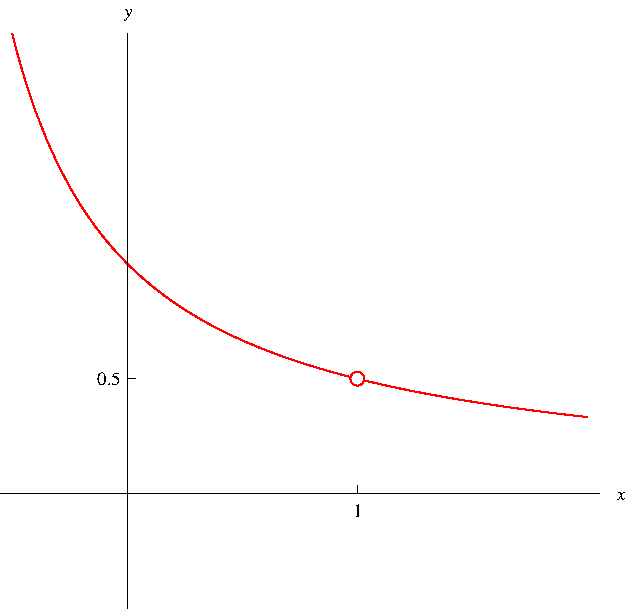
\includegraphics[height=4.5cm]{limits/pictures/02-01-ex1.pdf}%
}
\column{.5\textwidth}
\begin{itemize}
\item  Guess the value of $\lim_{x\rightarrow 1}\frac{x - 1}{x^2 - 1}$.
\item<2->  Notice that $\frac{x-1}{x^2-1}$ doesn't exist at $1$.  
\item<3->  It does exist at values near $1$.
\item<5->  We guess that the limit is $0.5$. 
\item<6->  In this case, our guess is correct.
\end{itemize}
\end{columns}
\uncover<4->{
\[
\begin{array}{|r@{.}l|r@{.}l||r@{.}l|r@{.}l|}
\hline
\multicolumn{2}{|c|}{x} &
\multicolumn{2}{|c||}{f(x)} &
\multicolumn{2}{|c|}{x} &
\multicolumn{2}{|c|}{f(x)} \\
\hline
0 & 
5 & 
0 & 
666667 & 
1 & 
5 & 
0 & 
400000 \\ 
0 & 
9 & 
0 & 
526316 & 
1 & 
1 & 
0 & 
476190 \\ 
0 & 
99 & 
0 & 
502513 & 
1 & 
01 & 
0 & 
497512 \\ 
0 & 
999 & 
0 & 
500250 & 
1 & 
001 & 
0 & 
499750 \\ 
0 & 
9999 & 
0 & 
500025 & 
1 & 
0001 & 
0 & 
499975 \\ 
\hline
\end{array}
\]
}
\end{example}
\end{frame}
% end module limit-ex1
